%  !TeX  root  =  user_guide.tex 

%\subsection{OGR Converter Plugin}
\section{Extension Convertisseur de couche OGR}

% when the revision of a section has been finalized, 
% comment out the following line:
%\updatedisclaimer

%The OGR Layer Converter plugin adds the ability to convert vector data from one OGR-supported 
%vector format to another.\footnotetext{Supported formats may vary according to the installed 
%GDAL/OGR package.}
%The plugin is very simple to run, and only requires a few parameters to be 
%specified before running:
L'extension Convertisseur de couche OGR offre la possibilité de convertir des 
données vectorielles possédant un format supporté par la librairie OGR vers 
un autre format vectoriel supporté.\footnotetext{Les formats supportés 
peuvent varier en fonction de la version de librairie GDAL/OGR installée.}
Cette extension est très simple à mettre en \oe uvre et ne requiert que 
quelques réglages avant son exécution:

%\begin{itemize}
%\item \textbf{Source Format/Datset/Layer}: Enter OGR format and path to the vector file to be converted
%\item \textbf{Target Format/Datset/Layer}: Enter OGR format and path to the vector output file
%\end{itemize}
\begin{description}
\item[Source Format/Jeu de données/Couche :] Spécifier le format OGR 
ainsi que l'emplacement de stockage du fichier vecteur à convertir
\item[Cible Format/Jeu de données/Couche :] Spécifier le format OGR 
ainsi que l'emplacement de sauvegarde du fichier vecteur convertit
\end{description}

%\begin{figure}[ht]
%   \begin{center}
%   \caption{OGR Layer Converter Plugin \nixcaption}\label{fig:ogr_converter_dialog}\smallskip
%   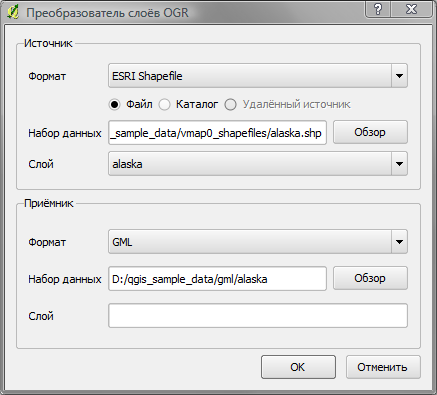
\includegraphics[clip=true, width=7.5cm]{ogr_converter_dialog}
%\end{center}  
%\end{figure}
\begin{figure}[ht]
   \centering
   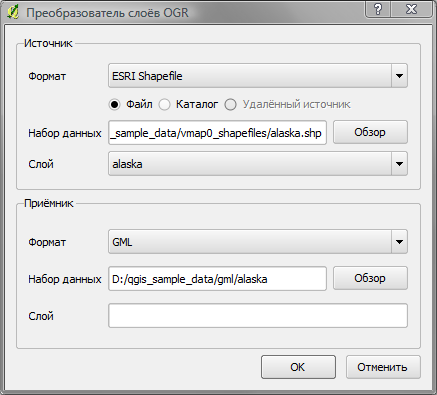
\includegraphics[clip=true, width=7.5cm]{ogr_converter_dialog}
   \caption{L'extension Convertisseur de couche OGR \nixcaption}\label{fig:ogr_converter_dialog}
\end{figure}

%\minisec{Using the Plugin}
\minisec{Mettre en \oe uvre l'extension}

%\begin{enumerate}
%  \item Start QGIS, load the OGR converter plugin in the Plugin Manager (see Section 
%  \ref{sec:load_core_plugin}) and click on the \toolbtntwo{ogr_converter}{OGR Layer Converter} 
%  icon which appears in the QGIS toolbar menu. The OGR Layer Converter plugin dialog appears as shown in Figure \ref{fig:ogr_converter_dialog}.
%  \item Select the OGR-supported format (e.g., \selectstring{ESRI Shapefile}{\ldots}) and the path to the vector input file (e.g., \filename{alaska.shp}) in the Source area.
%  \item Select the OGR-supported format (e.g., \selectstring{GML}{\ldots}) and define a path and the vector output filename (e.g., \filename{alaska.gml}) in the Target area.
%  \item Click \button{Ok}.
%\end{enumerate}
\begin{enumerate}
  \item Lancez \qg, activez l'extension Convertisseur de couche OGR depuis le 
  Gestionnaire d'Extensions (voir la Section \ref{sec:load_core_plugin}) puis 
  appuyez sur l'icône\\ \toolbtntwo{ogr_converter}{Lancer le Convertisseur de couche OGR} 
  qui apparaît dans la barre d'outils QGIS. La boîte de dialogue de 
  l'extension Convertisseur de couche OGR apparaît alors comme montré dans la 
  Figure \ref{fig:ogr_converter_dialog}.
  \item Dans le bloc Source, spécifiez le format OGR supporté (par exemple,\\ \selectstring{ESRI Shapefile}{\ldots}) 
  ainsi que l'emplacement de stockage du fichier vecteur à convertir (par exemple, \filename{alaska.shp}).
  \item Dans le bloc Cible, spécifiez le format OGR de sortie (par exemple, \selectstring{GML}{\ldots}) 
  et choisissez un nom ainsi qu'un emplacement de sauvegarde pour le fichier 
  convertit (par exemple, \filename{alaska.gml}).
  \item Appuyez sur \button{Ok}.
\end{enumerate}